\subsection[Implementation of Guarding Algorithms]{Implementation of Polygon Guarding Algorithms for Art Gallery Problems}
Maleki and Mohades \cite{maleki2022implementation} introduce their implementations for two existing approximation algorithms (\cite{GHOSH2010718}, \cite{bhattacharya2016approximability}) for computing visibility in simple polygons. Additionally, they develop their own visibility algorithm. They lastly  evaluate experimentally their implementations for the three algorithms in the context of the Art Gallery Problem \cite{o1987art}.

To begin with, we will introduce some terminology used throughout this summary. The algorithms distinguish in their implementation between vertex guards and point guards in  a polygon $P$. Vertex guards can be placed only on the vertices of $P$. Point guards can be placed without restriction inside $P$. Lastly, the algorithms are tested on weak visibility polygons. A polygon $P$ has weak visibility if all boundary vertices of $P$ can see all the points in $P$.

% Given that computing a minimum number of guards for guarding a polygon is NP-hard \cite{1057165}, Maleki and Mohades inspect how the Art Gallery Problem \cite{o1987art} can be tackled using three approximation algorithms.

\subsubsection{Algorithm of Ghosh}
The algorithm of Ghosh \cite{GHOSH2010718} runs in $O(n^4)$ time and yields an $O(\log n)$-approximation algorithm for computing the minimum vertex guard for simple polygons. 

One of the most important concepts the algorithm works with is that of a convex component. Given a polygon $P$, we can form subsets of the vertices in $P$ such that all the subsets form convex subpolygons of $P$. We call these subsets of vertices the convex components of $P$.

The algorithm begins by computing the set of all the convex components $C$ of a given polygon $P$. Then, each vertex $j \in P$ creates a set $F_j$ with the convex components from $C$ that it is able to fully see. Let $F := \{F_j | \forall j \in P, F_j \subseteq C \text{ seen by } j\}$. Then, the algorithm checks for overlaps between the sets of $F$. For every vertex $i$ and its corresponding convex components set $F_i$, the algorithm checks whether any of the other sets $F \setminus F_i$ sets are included in $F_i$. That is, if $F_j \subseteq F_i, F_j \in F, i \neq j$. If that is the case, then  vertex $i$ sees at least as little as $j$. The vertex $j$ is thus not needed as a guard, so $F_j$ is removed from $F$. Vertex $i$ is added in the final guard set $S$. The algorithm repeats until the set $F$ becomes empty. When that happens, it means that the algorithm found a set $S$ of guards who see all the convex components of $P$ without overlap.

% The redundant sets $F_j, \forall j$ are afterwards eliminated as follows: for all fixed $j$, the algorithm searches for a vertex $i \neq j, i \in P$ such that $F_i$ is also visible from $j$ ($|F_i| \leq |F_j|$); $F_i$ is eliminated, $j$ is added to $S$ and the process continues until $C$ is empty. At the end, $S$ contains the approximated guard set for $P$.

An example run of the algorithm is depicted in Figure \ref{fig:ghosh}. Let $P$ be the polygon in question, and its boundary vertices $\mathcal V = \{1, 2, 3, 4, 5, 6\}$. Polygon $P$ is divided into two convex components $C_1$ and $C_2$, such that $C = \{C_1, C_2\}$. The sets $F_j, \forall j \in P$ are also displayed. Since $F_1 \subseteq F_2 \subseteq F_3 \subseteq F_4 \subseteq F_6$ and $F_5 \subseteq F_3 \subseteq F_4 \subseteq F_6$, $F_1, F_2, F_3, F_4$, and $F_5$ are removed. The remaining set $F_6$ yields the final guard set $S = \{6\}$, which can see both convex regions of $P$, and hence the whole polygon.

\begin{figure}[h!]
    \centering
    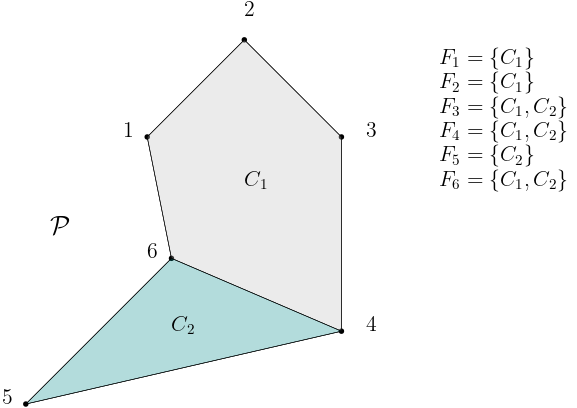
\includegraphics[width=0.7\textwidth]{literature/ghosh-eg.png}
    \caption{Example run of the Algorithm of Ghosh \cite{GHOSH2010718} with polygon $P$ divided into two convex components $C_1$ and $C_2$. The resulting guard set is $S = \{6\}$}
    \label{fig:ghosh}
\end{figure}

\newpage
\subsubsection{Algorithm of Bhattacharya, Ghosh and Roy}
The algorithm of Bhattacharya et al. \cite{bhattacharya2016approximability} runs in $O(n^2)$ time and yields a 6-approximation for computing the minimum vertex guard for weak visibility polygons without holes. 

It begins by choosing two neighbours $u$ and $v$ as parents for every vertex in $P$. It then computes the Shortest Path from each pair of parents $(u, v)$ to every other vertex in $P$. The Shortest Path is a path between two vertices such that the distance between them is minimal. If all distances between two adjacent vertices are the same, then the length of the path corresponds to the number of edges between the vertices. The Shortest Path from a pair of vertices $(u, v)$ to any other vertex $w$ is the length of the minimum path between $u$ and $w$, and $v$ and $w$.

Then, all vertices that can be reached from $u$ and $v$ are unmarked. In increasing angular order from $\overline{uv}$, every vertex $w \in P$ is checked for visibility from $u, \text{ and } v$. If all vertices $w$ are visible, then $u, \text{ and }v$ are added to $S$. Otherwise, $w$ is added to $S$ and the procedure continues with $w$ as the starting node. All vertices that become seen from $S$ are marked. At the end, the algorithm checks whether the vertices in $S$ have overlapping visibility regions, and duplicates are removed.

An example run of the algorithm is depicted in Figure \ref{fig:bhaca}. Let $P$ be the polygon in question, and its boundary vertices $\mathcal V = \{a, b, c, d, e, f\}$. The algorithm starts with vertices $a$ and $c$ as parents of $b$. Clockwise, vertex $d$ is visible from $\overline{ac}$, but $e$ is not. For this reason, $e$ is added to the guard set $S$, and vertices $d$ and $f$ are chosen as the new parents. In increasing angular order, all vertices $a, b, c, e$ are visible from $\overline{ef}$, so $d$ and $f$ are added to $S$. Since the visibility regions of $d$ and $f$ coincide ($Vis(d) = Vis(f)$), and the visibility region of $e$ is included in that of $d$ and $f$ ($Vis(e) \subseteq Vis(d) \subseteq Vis(f)$), $e$ and $d$ can be removed from $S$. As such, the final guard set becomes $S = \{f\}$.

\begin{figure}[h!]
    \centering
    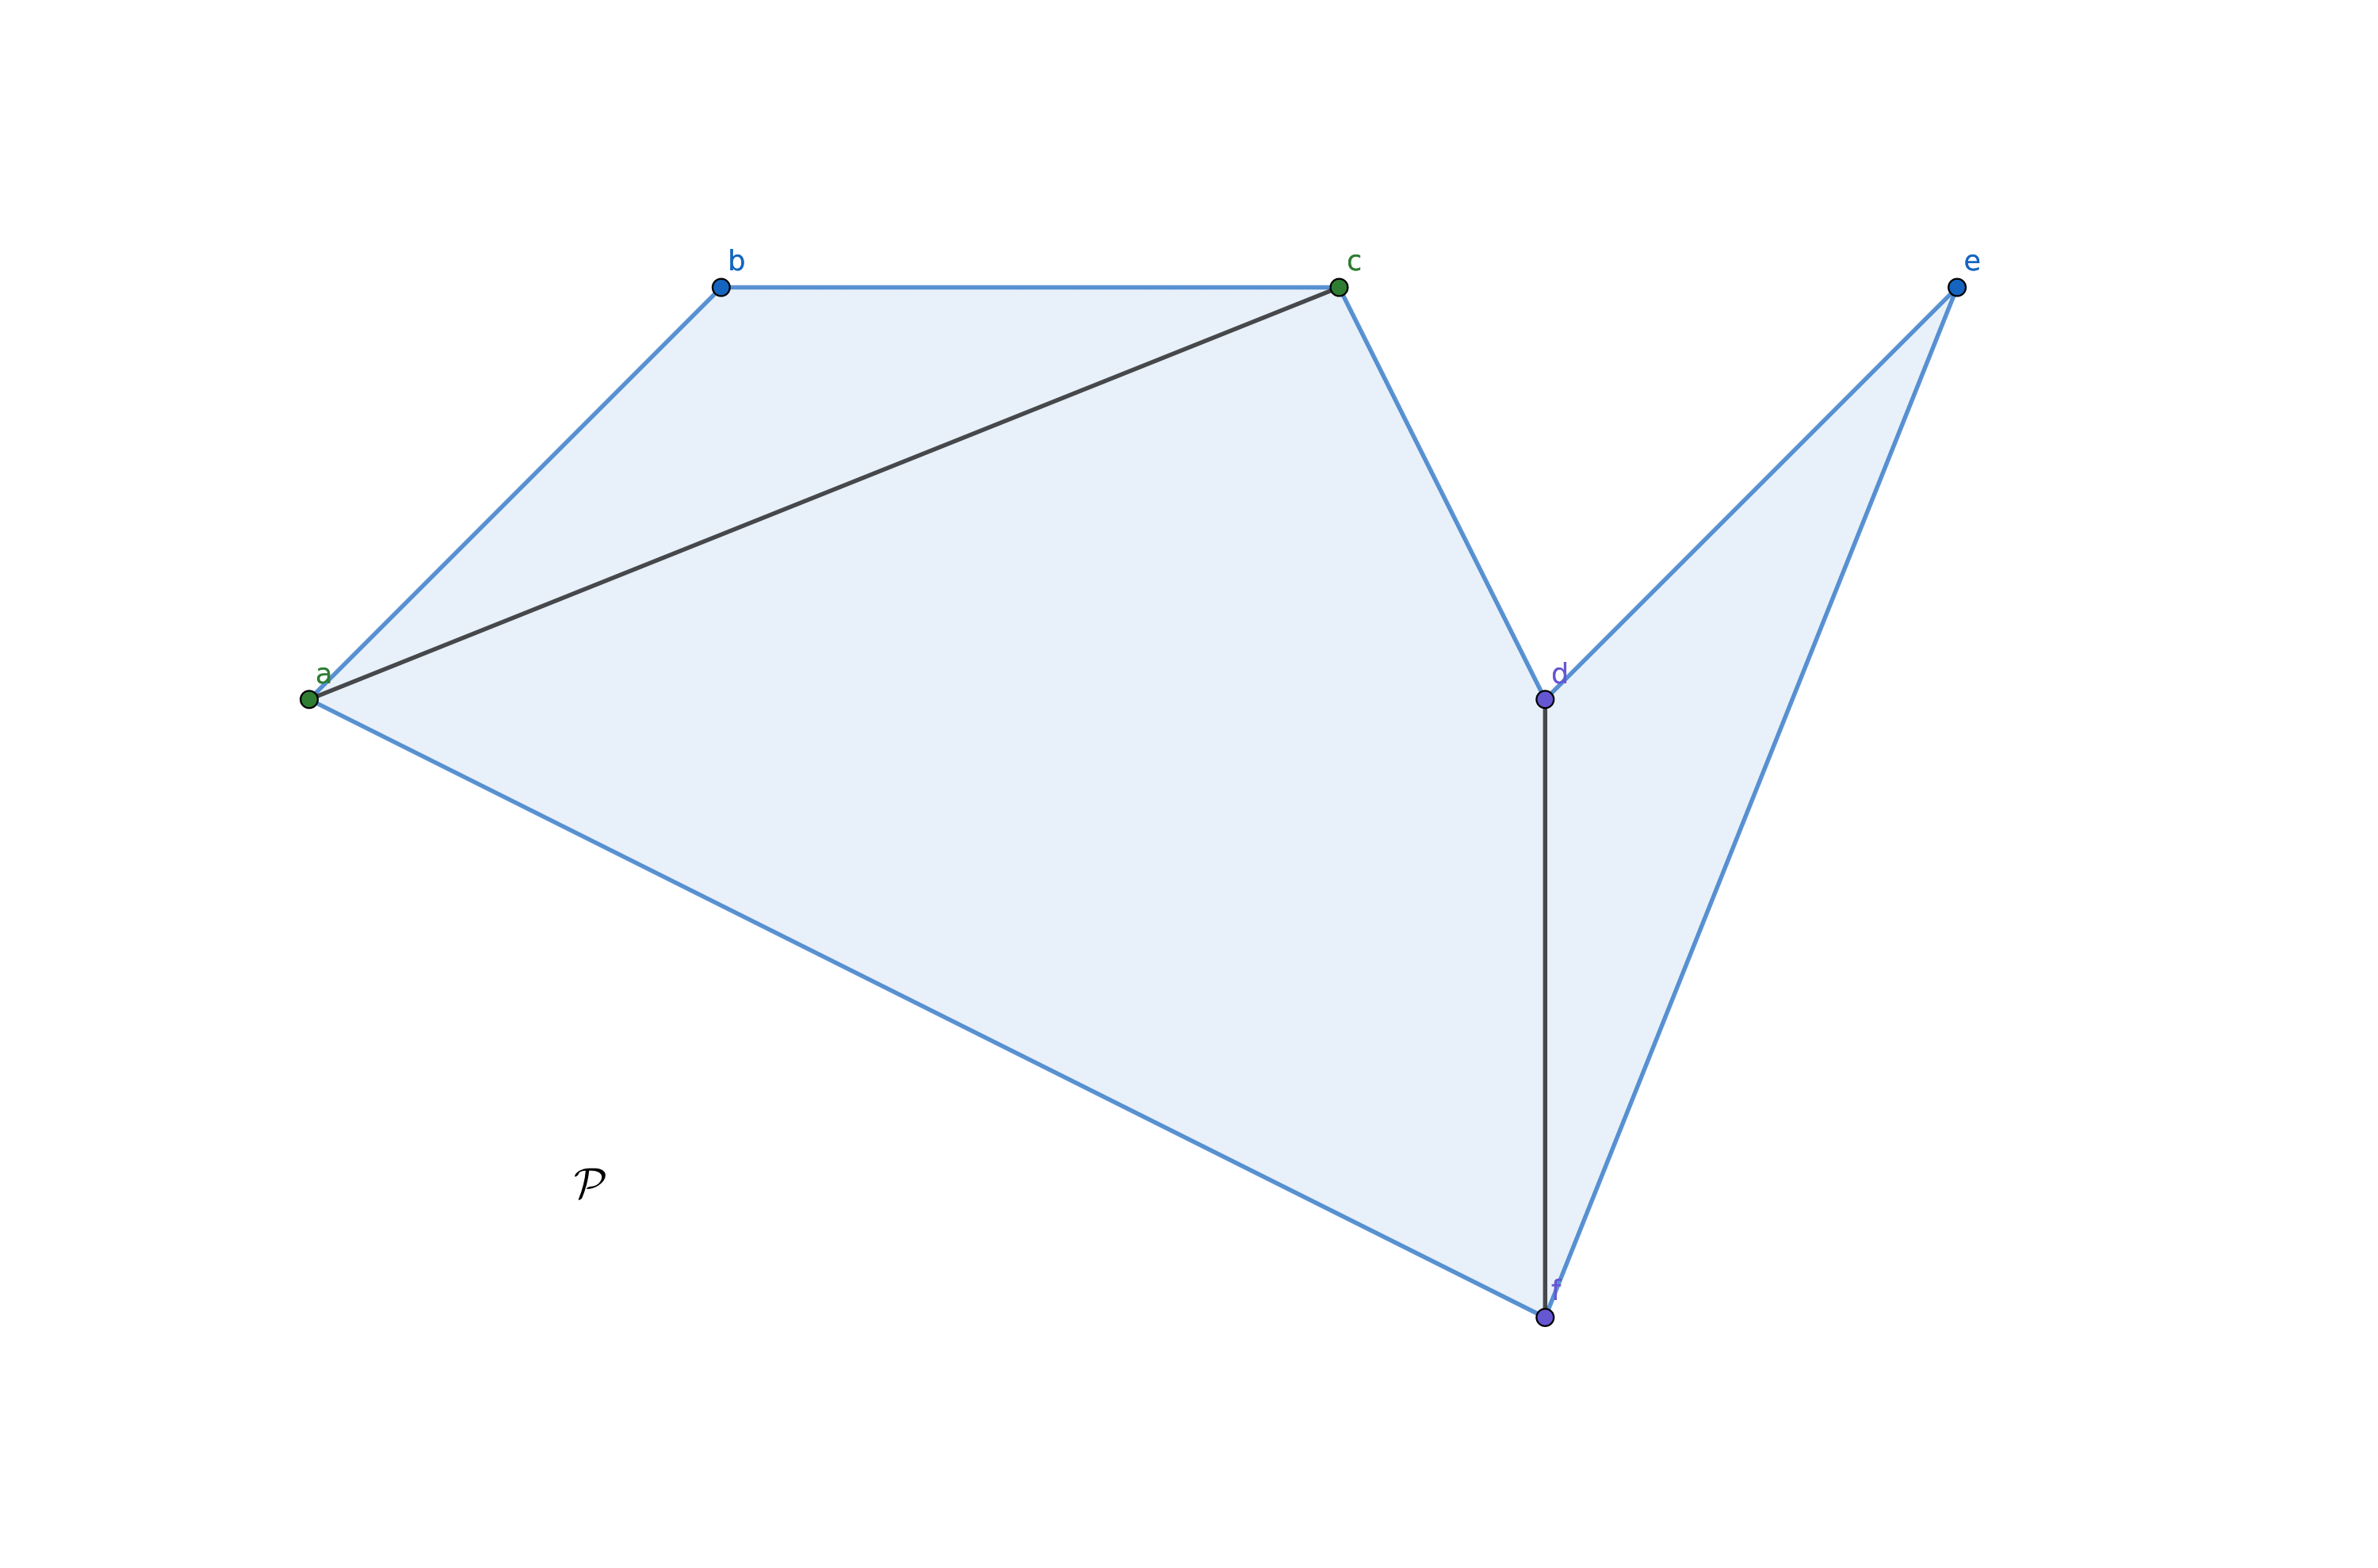
\includegraphics[width=0.5\textwidth]{literature/bacha-eg.png}
    \caption{Example run of the Algorithm of Bhattacharya et al. \cite{bhattacharya2016approximability} for polygon $P$. The final guard set is $S = \{f\}$.}
    \label{fig:bhaca}
\end{figure}

\newpage
\subsubsection{New Algorithm}
The algorithm introduced by Maleki and Mohades is focussed on polygons with large number of vertices $n$ and different amounts of reflex vertices $r$. If the number of reflex vertices is significantly lower than the total number of vertices ($r \leq \log \log n$), guards are placed at all reflex vertices. Otherwise, they are placed according to the algorithm of Ghosh \cite{GHOSH2010718}.

\subsubsection{Experiments}
Algorithms of Ghosh \cite{GHOSH2010718} and Bhattacharya et al. \cite{bhattacharya2016approximability} are tested on weak visibility polygons, and the newly introduced algorithm is tested on simple polygons. 

Let Procedure 1 be a procedure for generating weak visibility polygons that is illustrated in Figure \ref{fig:weak}: given two points $p = (k, 0), q = (-k, 0)$,  $n$ random points $\{x_1, ..., x_n\}$ sorted on the distance from $p$ on $\overline{pq}$, $n$ sorted random angles $\{\alpha_1, ..., \alpha_n\} \in  (0, \pi)$, and $n$ vertices $\{y_1, ..., y_n\}$ are created by shooting $n$ rays at the corresponding angle $\alpha_i, \forall x_i$. Then, $n$ reflex vertices $\{z_1, ..., z_n\}$ are added in the quadrilateral formed by vertices $x_iy_iy_{i + 1}x_{i + 1}$. The figure is accredited to \cite{maleki2022implementation}.

\begin{figure}[h!]
    \centering
    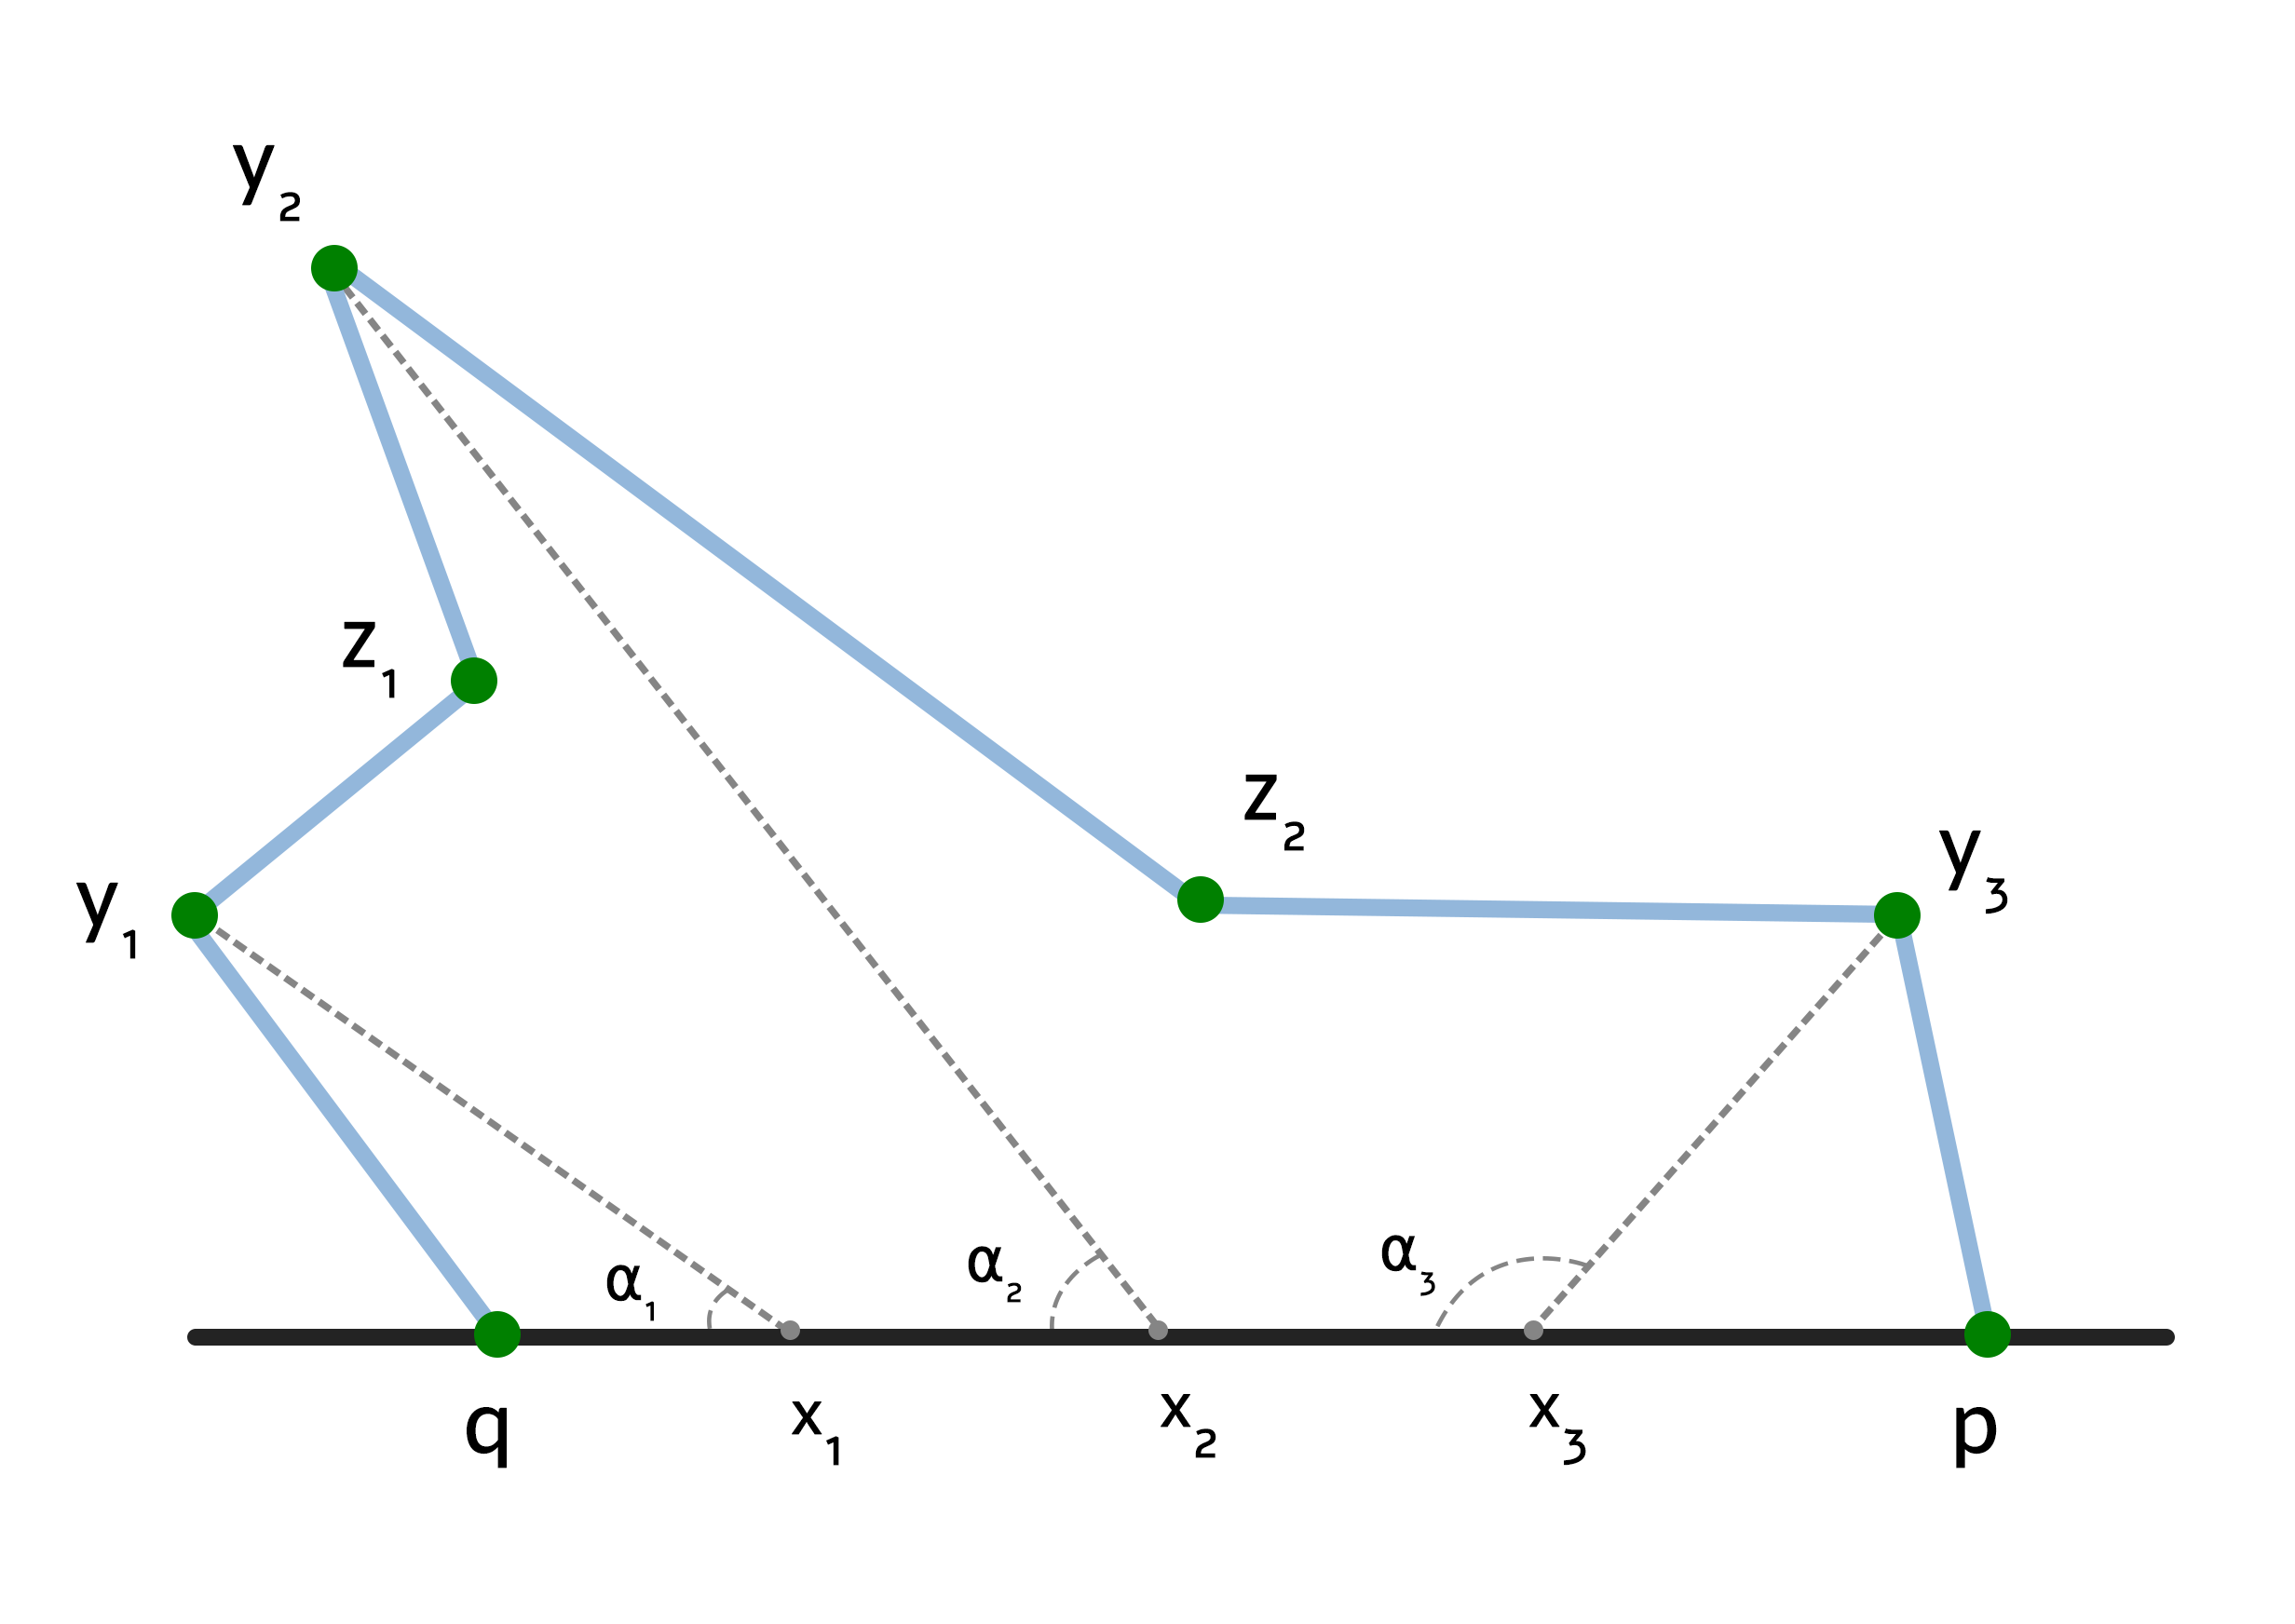
\includegraphics[width=0.6\textwidth]{literature/weak.png}
    \caption{Generated weak visibility polygon for $n = 3$ \cite{maleki2022implementation} through Procedure 1.}
    \label{fig:weak}
\end{figure}

The algorithms of Ghosh \cite{GHOSH2010718} and Bhattacharya et al. \cite{bhattacharya2016approximability} were tested using polygons generated by Procedure 1 with $n \in \{10, 11, ..., 15\}$ vertices and $r \in \{2, 3\}$ reflex vertices. The results suggest that for low values of $n$ and $r$, the algorithm of Ghosh \cite{GHOSH2010718} performs better when using the number of guards as evaluation criteria. 
% Its constant time approximation in the small case contrasts with the constant approximation of the algorithm of Bhattacharya \cite{bhattacharya2016approximability}.
Similarly, the algorithm of Ghosh \cite{GHOSH2010718} performed better both when tested on a weak visibility polygon with low $n = \overline{10, 15}$ and $\frac n 2 \leq r$, and when tested with large $n \in \{100, 400\}$.

Secondly, let Procedure 2 be a procedure for generating simple polygons with custom number of reflex vertices $r$ is devised in Figure \ref{fig:arbitrary}. The figure was taken from \cite{maleki2022implementation} and annotated to suit the explanations in these summaries. Starting from a simple convex polygon $P$ with $n$ vertices ($u, v, x1, x2, ..., x7$), $P$ is triangulated such that every triangle has a joint edge with its boundaries; $r$ reflex vertices ($r1, r2, r3$) are randomly added inside $P$, and the boundaries outside of the reflex vertices are moved such that all $r$ points are now forming boundaries. 

\begin{figure}[h!]
    \centering
    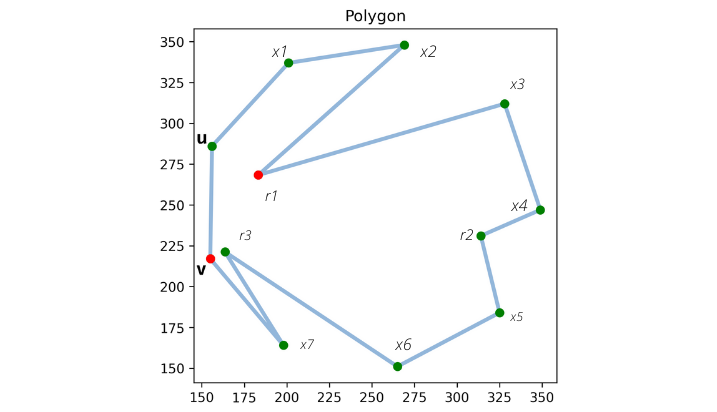
\includegraphics[width=0.7\textwidth]{literature/concave_test.png}
    \caption{Generated simple polygon $P$ for $n = 12, r = 3$ \cite{maleki2022implementation} through Procedure 2.}
    \label{fig:arbitrary}
\end{figure}

The new algorithm is tested on simple polygons constructed as mentioned by starting from low $r$ and gradually increasing it. The results are reported positively in the sense that the $|S|$ always remains close to the optimal, as a 2-approximation solution.

Therefore, through the newly implemented algorithm, Maleki and Mohades \cite{maleki2022implementation} testify that the algorithm of Ghosh \cite{GHOSH2010718} performs like a constant approximation in practice, and often better than its theoretical bound when tested on complex simple polygons.
% - guards placed on vertices = vertex guards
% - no restrictions = point guards
% - $P$ is called weak visibility polygon if every point in $P$ is visible from some point of an edge
% - the problem of computing a min number of guards is NP-hard
% - $O(n^4)$ approximation algorithm for computing $S$ (1)
% - $O(n^2)$ 6-approximation algorithm for vertex \subsection{Implementation of Polygon Guarding Algorithms for Art Gallery Problems \cite{maleki2022implementation}}
% - guards placed on vertices = vertex guards
% - no restrictions = point guards
% - $P$ is called weak visibility polygon if every point in $P$ is visible from some point of an edge
% - the problem of computing a min number of guards is NP-hard
% - $O(n^4)$ approximation algorithm for computing $S$ (1)
% - $O(n^2)$ 6-approximation algorithm for vertex guarding a weak vibisility $P$ with no holes (2)
% - implementation of algorithms and testing on weak visibility polygons
% - generating arbitrary weak visibility polygons *add algorithm* and testing them with $n = \overline{10, 15}$ and $r \in \{2, 3\}$ reflex vertices
	% - for low value of $n$ and $r$, it is better to use Algorithm 1 for minimising the number of vertex guards; since algorithm 2 is a constant approximation algorithm, algorithm 1 performs like a constant time approximation algorithm for small values of $n$ and $r$ experimentally
	% - since the criteria of minimisation is the number of guards rather than the running time which is a one-time affair unlike online algorithms, algorithm 1 is preferable even for weak visibility polygons
% - generating arbitrary weak visibility polygons and testing them with $n = \overline{10, 15}$ and $r$ reflex vertices close to the number of convex vertices
	% - for a low value of $n$ and $\frac n 2 \leq r$, algorithm 1 is better for guarding a weak visibility polygon with a min number of guards, because when the number of reflex vertices increases, the number of the diameter of the polygon and convex components decrease
% - generating arbitrary weak visibility polygons and testing them with large $n$
	% - algorithm 1 is better for guarding a weak visibility polygon with min number of guards, because it uses less guards than algorithm 2
% - generating arbitrary simply polygons *add algorithm* (Ghosh)
% - if $r << n$ , then the size of the optimal guard set is $\approx r$  => the number of edges $E$ in the visibility graph of such simple polygons is $O(n^2)$ => choose a small number $\log \log n$ as an upper bound for $r$ so that $r$ and optimal are close
% - if $r - c \leq \log \log n$, $c$ - small constant, then we place guards at all reflex vertices for guarding a simple polygon $P$, otherwise we place guards using the method of algorithm 1
% - even if $E$ reduces, the chosen guard sets remains close to the optimal and the algorithm assigns no more than twice the optimal number of guards
% => Ghosh's idea works better in practice and performs like a constant approximation algorithmalgorithm 2 is a constant approximation algorithm, algorithm 1 performs like a constant time approximation algorithm for small values of $n$ and $r$ experimentally
	% - since the criteria of minimisation is the number of guards rather than the running time which is a one-time affair unlike online algorithms, algorithm 1 is preferable even for weak visibility polygons
% - generating arbitrary weak visibility polygons and testing them with $n = \overline{10, 15}$ and $r$ reflex vertices close to the number of convex vertices
	% - for a low value of $n$ and $\frac n 2 \leq r$, algorithm 1 is better for guarding a weak visibility polygon with a min number of guards, because when the number of reflex vertices increases, the number of the diameter of the polygon and convex components decrease
% - generating arbitrary weak visibility polygons and testing them with large $n$
	% - algorithm 1 is better for guarding a weak visibility polygon with min number of guards, because it uses less guards than algorithm 2
% - generating arbitrary simply polygons *add algorithm* (Ghosh)
% - if $r << n$ , then the size of the optimal guard set is $\approx r$  => the number of edges $E$ in the visibility graph of such simple polygons is $O(n^2)$ => choose a small number $\log \log n$ as an upper bound for $r$ so that $r$ and optimal are close
% - if $r - c \leq \log \log n$, $c$ - small constant, then we place guards at all reflex vertices for guarding a simple polygon $P$, otherwise we place guards using the method of algorithm 1
% - even if $E$ reduces, the chosen guard sets remains close to the optimal and the algorithm assigns no more than twice the optimal number of guards
% => Ghosh's idea works better in practice and performs like a constant approximation algorithm